%!TEX root = ../disertace.tex
%!TEX encoding = UTF-8 Unicode

\chapter{\seman}
\label{sec:seman}
The annotation tool \seman\ is written in Perl 5\footnote{\url{www.perl.org}; \url{dev.perl.org/perl5}} with Perl/Tk\footnote{\url{PerlTk.org}} GUI toolkit. The annotation tool depends on working installation of \tred, specifically its unix installation, because it uses \texttt{nTrEd} for efficient execution of \tred\ scripts in the background. \texttt{nTrEd} however, unlike \tred\ itself or \texttt{bTrEd}, does not work on Windows.% because it uses unix sockets.

 \seman\ itself is composed of several parts:
\begin{itemize}
  \item A frontend loads an \sf, a \semlex,  and a log file for this \sf, if it had already been annotated. 
  \item \ntred\ backend that is used to 
	\begin{itemize}
	  \item generate surface sentences from tectogrammatical trees in \tf{}s that are then displayed in the \seman\ GUI,
	  \item perform all the on-the fly pre-annotations (\Sref{sec:annot:pre})
	\end{itemize}
  \item A \semlex\ module is used to read, save, and edit \semlex.
  \item There is of course also a suite of miscellaneous scripts mostly for validation of annotated data, comparing and merging multiple annotations, merging annotators' \semlex{}es and computing reliability of annotations.
\end{itemize}

\section{Annotation logs}
\label{sec:logs}


\section{User interface}
\label{sec:seman:gui}

\subsection{Key bindings}

% sem-ann screenshot 
\begin{figure}[htbp]
   \centering
   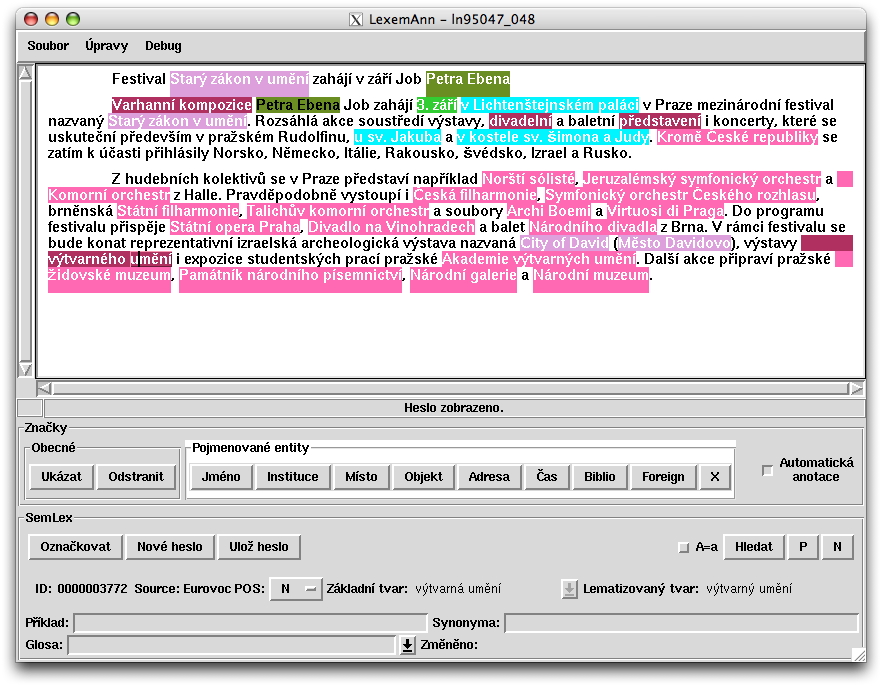
\includegraphics[scale=.4]{images/sem-ann.png} 
   \caption{An annotated document in \seman. the ``\code{sel}''-- selection tag is barely visible on the word \pr{umění} (second word from the left, second line from the bottom). The \semlex\ entry that is displayed in the Semlex-part of the UI -- \pr{výtvarná umění} -- is the one used to annotate the selected word. }
   \label{fig:example}
\end{figure}